\documentclass[12pt]{article}
%\usepackage[english]{babel}
\RequirePackage[spanish]{babel}
\usepackage[spanish]{babel}
\usepackage{graphicx}
%\usepackage[pdftex,bookmarks,colorlinks,breaklinks]{hyperref}  % PDF hyperlinks, with coloured links
%\usepackage[spanish]{babel}
\usepackage[pdftex,bookmarks,breaklinks]{hyperref}  % PDF hyperlinks, with coloured links
%\usepackage[spanish]{babel}
\usepackage[utf8]{inputenc}
\usepackage{epstopdf}
\usepackage{fullpage}
\usepackage{url}
\usepackage{colortbl}
\usepackage{lscape}
\usepackage{float}
\renewcommand{\baselinestretch}{1.5}
\usepackage{multirow}
\parskip 3ex % espacio entre parrafos.
\makeatletter
\renewcommand\paragraph{\@startsection{paragraph}{4}{\z@}%
	{-2.5ex\@plus -1ex \@minus -.25ex}%
	{1.25ex \@plus .25ex}%
	{\normalfont\normalsize\bfseries}}
\makeatother
\setcounter{secnumdepth}{4} % how many sectioning levels to assign numbers to
\setcounter{tocdepth}{4}    % how many sectioning levels to show in ToC

\begin{document}
%%%%%%%%%%%%%%% PORTADA %%%%%%%%%%%%%%%%%%
\pagestyle{empty}
\begin{figure}
   \centering
   
\includegraphics[scale=.5]{imgs/logo_utal.png}
\end{figure}

\begin{center}
Facultad de Ingeniería\\
Escuela de Ingeniería en Bioinformática\\
Ingeniería de Software\\
\bigskip\bigskip\bigskip\bigskip

\rule{14cm}{0.5mm}

\begin{Huge}\textbf{Título de informe}\end{Huge}

\rule{14cm}{0.5mm}

\bigskip\bigskip\bigskip\bigskip
\bigskip\bigskip\bigskip\bigskip
\bigskip\bigskip\bigskip\bigskip
%\bigskip\bigskip\bigskip\bigskip
%\bigskip\bigskip\bigskip\bigskip

\begin{tabular*}{14cm}{l@{\extracolsep{\fill}}r}
\textbf{\emph{Integrantes:}} & \textbf{\emph{Profesor:}}\\
Nombre Integrante1 & Nombre Profesor\\
Nombre Integrante2 & \textbf{\emph{Ayudante:}}\\
Nombre Integrante3 & Nombre Ayudante\\
\end{tabular*}
\end{center}

%%%%%%%%%%%%%%%%%%%%%%%%%%%%%%%%%%%%%%%
\newpage
\pagestyle{plain}
\tableofcontents

%%%%%%%%%%%%%%%%%%%%%%%%%%%%%%%%%%%%%%%
\newpage
\listoffigures 

%%%%%%%%%%%%%%%%%%%%%%%%%%%%%%%%%%%%%%%
\newpage
\listoftables


%%%%%%% INTRODUCCIÓN %%%%%%%%%%%%%%%%
\newpage
\section{Introducción}
\color{red}
La vida actual en la que vivimos está rodeada de aparatos tecnológicos y diversos elementos que han extendido la forma en que las personas interactúan entre ellas y con su entorno, dentro de estas interacciones es sencillo notar que existe un incremento en en interés de las personas en visitar lugares culturales como pueden centros históricos, lugares patrimoniales y museos (datos obtenidos de : SNM subdirección Nacional de Museos).

2019 - 1.210.075\\
2018 - 1.390.952 - 18.73 m\\
2017 - 1.252.418 - 18.47 m\\
2016 - 1.276.068 - 18.21 m\\
2015 - 1.112.809 - 17.97 m\\
2014 - 714.137 - 17.76 m\\
2013 - 719.675 - 17.57 m\\
2012 - 685.103 - 17.40 m\\
2011 - 632.765 - 17.23 m\\
2010 - 561.461 - 17.06 m\\
2009 - 682.144 - 16.89 m\\
2008 - 667.679 - 16.71 m\\
https://www.museoschile.gob.cl/sitio/Contenido/Institucional/90496:Estadisticas-generales\\
\color{black}

\subsection{Propósito}
\color{red}
Este proyecto está dirigido a todo público, enfocado en amantes de la cultura y aficionados por la realidad aumentada.
El propósito de esta aplicación es conectar por esta nueva vía a las personas con los museos locales, acercandolos hasta sus propias manos.
 en el siguiente documento se documenta el diseño de la aplicación en conjunto a su plan de desarrollo desde la concepción de la idea hasta la implementación y mantenimiento de esta.

\color{black}

\subsection{Descripción breve del problema}
\color{red}
(posible problema) el COVID-19 a traído consigo grandes cambios con respecto a cómo es nuestro estilo de vida, y generando para la mayoría de la población mundial el tener que adaptarse y usar aun mas de lo que ya se usaban la tecnología para poder conectarse con el resto de personas,  junto con esta adaptación también debemos destacar que cosas como salir de la casa para ir al colegio o salir de la casa a en un paseo familiar se transformaron en actividades que no están permitidas. (datos del gob de chile ->) podemos notar con los datos del gob la gran baja en la asistencia a los museos desde marzo del 2020 en chile (insertar cifra), este fenómeno ha alejado a los museos de las personas que podrían estar interesadas.

\color{black}

%%%%%%% PLANIFICACIÓN DE TRABAJO %%%%%%%%%%%%
\newpage
\section{Planificación del Trabajo}

\subsection{Descripción del grupo de trabajo}
El grupo para este proyecto esta conformado por:

\begin{longtable}{|c|c|c|}
\hline 
Nombre & Alias & Capacidades de profesión \\ 
\hline 
José Rojas & JR & Programador Junior, Artista, Diseñador de Videojuegos \\ 
\hline 
Nicolás Romero & NR & Programador Junior, Artista, Diseñador de Videojuegos \\ 
\hline 
\end{longtable} 

Descripción del general del trabajo de JR: Se encargará de la gestión del proyecto, el
plan del proyecto, trabajara en conjunto con su compañero para hacer los requerimientos,
realizara tanto el diseño inicial como detallado de la app, hará la mitad de la codificación y por ultimo hará la creación de la UI.

Descripción del general del trabajo de NR: Se encargará de parte de los requerimientos,
trabajara en conjunto con su compañero para hacer el plan del proyecto,ademas realizara la
prueba unitaria, prueba funcional, prueba de integración, prueba de la aplicación finalizada
y por ultimo, hara la mitad de la codificación del proyecto y la creación de Assets 3D.


\subsection{Estimación de esfuerzo}
En la siguiente sección se especifica la estimación de esfuerzo para la realización de esta app tomando en cuenta los las diferentes entradas y complejidades de archivo además de sus costes de producción.

\subsubsection{Complejidad de Archivos}
La siguiente tabla muestra las diferentes funciones necesaria para el correcto funcionamiento del software.

\begin{longtable}{|p{5cm}|p{8cm}|}
\hline 
Tipos de parámetros & Nombres \\ 
\hline 
EI (Entradas Externas) & Obtener Pieza Historica (PH), Buscar PH \\ 
\hline 
EO (Salidas Externas) & Compartir Modelo 3d o Foto de PH en RRSS.
Lista de piezas historicas obtenidas, Biblioteca de trofeos obtenidos.
 \\ 
\hline 
EQ (Consultas Externas) & Visualizar PH, Rotar PH, Ver información de PH, Hacer Zoom in a PH, Hacer Zoom out a
PH.
 \\ 
\hline 
ILF (Ficheros lógicos internos) & Datos de PH, Datos de Trofeos. \\ 
\hline 
EIF (Ficheros de interfaces externas) & Obtener piezas historicas compartidas en
RRSS.
 \\ 
\hline 
\end{longtable} 

\begin{longtable}{|p{5cm}|p{8cm}|}
\hline 
Objetos & Datos necesarios \\ 
\hline 
Pieza Historica & Autor,Nombre de la pieza, Año de creación, Material
usado, dimensiones, Ubicación en el museo, Nombre del
Museo. Nombre del fotografo de la pieza. Detalles de la
pieza y datos interesantes. \\ 
\hline 
Trofeo & Tipo de Trofeo, Nombre de trofeo, detalles de trofeo. \\ 
\hline 
Museo & Nombre, ubicación, fecha de construcción, lista de piezas
historicas. \\ 
\hline 
\end{longtable} 

\subsubsection{Complejidad de las funcionalidades, cálculo de FP, grados de influencia, y otros cálculos}
En las siguientes tabla se muestra la complejidad de las diferentes funcionalidades ligadas al software.

\begin{longtable}{|c|c|c|c|}
\hline 
Entradas Externas EI &   &   &   \\ 
\hline 
Nombre & DET & FTR & Complex \\ 
\hline 
Obtener Pieza Historica & 4 & 1 & Low \\ 
\hline 
Buscar Pieza Historica & 2 & 1 & Low \\ 
\hline 
Obtener Trofeo & 3 & 1 & Low \\ 
\hline 
Escanear Codigo QR del Muse & 3 & 1 & Low \\ 
\hline 
\end{longtable}

\begin{longtable}{|c|c|c|c|}
 \hline 
 Salidas Externas EO &   &   &   \\ 
 \hline 
 Nombre & DET & FTR & Complex \\ 
 \hline 
 Compartir Modelo 3d o Foto de PH en RRSS & 3 & 2 & Low \\ 
 \hline 
 Biblioteca de piezas historicas obtenidas & 3 & 1 & Low \\ 
 \hline 
 Biblioteca de trofeos obtenidos. & 3 & 1 & Low \\ 
 \hline 
 \end{longtable}
 
 \begin{longtable}{|c|c|c|c|}
  \hline 
  Consultas Externas EQ &  &  &  \\ 
  \hline 
  Nombre & DET & FTR & Complex \\ 
  \hline 
  Visualizar Pieza Historica & 2 & 1 & Low \\ 
  \hline 
  Rotar Pieza Historica & 2 & 1 & Low \\ 
  \hline 
  Ver info. de Pieza Historica & 2 & 1 & Low \\ 
  \hline 
  Zoom in a Pieza Historica & 2 & 1 & Low \\ 
  \hline 
  Zoom out a Pieza Historica & 2 & 1 & Low \\ 
  \hline 
  Ver info. de Museo & 2 & 1 & Low \\ 
  \hline 
  Visualizar Museo & 2 & 1 & Low \\ 
  \hline 
  Ver info. de Trofe & 2 & 1 & Low \\ 
  \hline 
  \end{longtable} 
  
  \begin{longtable}{|c|c|c|c|}
   \hline 
   Ficheros lo´gicos internos ILF &  &  &  \\ 
   \hline 
   Nombre & DET & FTR & Complex \\ 
   \hline 
   Datos de Piezas Historicas & 11 & 1 & Low \\ 
   \hline 
   Datos de Trofeos & 4 & 1 & Low \\ 
   \hline 
   Datos de Museos & 4 & 2 & Low \\ 
   \hline 
   \end{longtable}  
   
   \begin{longtable}{|c|c|c|c|}
   \hline 
   EIF (Ficheros de interfaces externas) &  &  &  \\ 
   \hline 
   Nombre & DET & FTR & Complex \\ 
   \hline 
   Obtener piezas historicas compartidas en RRSS. & 3 & 2 & Low \\ 
   \hline 
   \end{longtable} 
   
   Ahora podemos calcular los puntos de función sin ajustar, TUFP.
   
   \begin{longtable}{|p{3cm}|p{1.5cm}|p{1.9cm}|p{1.5cm}|p{1.9cm}|p{1.5cm}|p{1.9cm}|}
   \hline 
     & \multicolumn{2}{c|}{Bajo} & \multicolumn{2}{c|}{Medio} & \multicolumn{2}{c|}{Alto} \\ 
   \hline 
     & Número & Puntuación & Número & Puntuación & Número & Puntuación \\ 
   \hline 
   Ficheros Lógicos Internos a la Aplicación & 3 & 7 & 0 & 10 & 0 & 15 \\ 
   \hline 
   Ficheros Lógicos Externos a la Aplicación
    & 1 & 5 & 0 & 7 & 0 & 10 \\ 
   \hline 
   Input Externos & 4 & 3 & 0 & 4 & 0 & 6 \\ 
   \hline 
   Outputs Externos
    & 3 & 4 & 0 & 5 & 0 & 7 \\ 
   \hline 
   Queries & 7 & 3 & 0 & 4 & 0 & 6 \\ 
   \hline 
     &   & 71 &   & 0 &   & 0 \\ 
   \hline 
   \end{longtable} 
   
   El total de TUFP = 53 , cálculo y tabla generada a partir de la planilla de cálculo.
   
   Grados de influencia y otros cálculos
   
   Calculamos los grados de influencia a partir de la planilla de calculo y podemos obtener lo siguiente:
   
   \begin{longtable}{|c|c|}
   \hline 
   TOTAL GRADOS DE INFLUENCIA & 11 \\ 
   \hline 
   Puntos de Función Ajustados & 53 \\ 
   \hline 
   VAF & 0,76 \\ 
   \hline 
   \end{longtable} 
   
\subsubsection{C.T Jones / COCOMO II}

\begin{longtable}{|c|c|}
\hline 
FP & 53 \\ 
\hline 
Loc en POO  & 20 \\ 
\hline 
\end{longtable} 

\begin{longtable}{|p{8cm}|c|}
\hline 
C.T Jones &   \\ 
\hline 
Métrica  & Cálculo \\ 
\hline 
Estimación de meses de desarrollo & 4,894522709 \\ 
\hline 
Número de personas necesarias para el desarrollo (NP) & 0,3533333333 \\ 
\hline 
Estimación del esfuerzo en personas/mes  & 1,729398024 \\ 
\hline 
Estimación de esfuerzo en horas hombre (160 horas x mes) 160 horas, ya que
, se considera 1 jornada diaria de 8 horas & 276,7036838 \\ 
\hline 
\end{longtable} 

Estimación de esfuerzo en base a C.T. Jones 1.996 Software Estimating Rules of Thumb” y B. Boehm COCOMO II en fase de Early Design

\begin{longtable}{|c|c|}
\hline 
COCOMO II &   \\ 
\hline 
Métrica  & Cálculo \\ 
\hline 
Conversión de FP a LOC. & 1060 \\ 
\hline 
\end{longtable}

Calculo de esfuerzo con COCOMO II con entrada de 1260 LOC y con factores de escala nominales.

\begin{longtable}{|p{3cm}|c|c|c|}
 \hline 
 Estimación & Optimista & Conservador & Pesimista \\ 
 \hline 
 Meses de desarrollo & 4,6 & 5,2 & 5,9 \\ 
 \hline 
 Personas necesarias & 0,4 & 0,6 & 0,8 \\ 
 \hline 
 Personas/mes & 2 & 3 & 4,5 \\ 
 \hline 
 Esfuerzo en horas hombre (160 horas x mes) & 294,4 & 499,2 & 755,2 \\ 
 \hline 
 \end{longtable}
 
\begin{longtable}{|c|c|}
  \hline 
  LOC Equivalentes & 1060 \\ 
  \hline 
\end{longtable}

Estimación del costo monetario en base al esfuerzo en HH conservador. Definiremos 2 perfiles:

Programador Junior: Perfil requerido para realizar la codificación crítica en base al diseño del software, gestión del proyecto, requerimientos, el plan del proyecto y los diseños base de la aplicación.

Artista Junior: Perfil requerido para la creación de assets 3d y UI para los diseños creados para el proyecto.

Estimación del coste de producir el software en 5.2 meses con 499 HH, bajo el modelo conservador de COCOMO II 

\subsection{Asignación de recursos}

\begin{longtable}{|p{4cm}|p{2.2cm}|p{2.4cm}|p{2.7cm}|p{2cm}|}
\hline 
Costo del producto  &   &   &   &   \\ 
\hline 
Etapa    & Distribución en \% & Distribución de T (HH) & Costo x Recurso & Recurso \\ 
\hline 
Gestión del proyecto & 3 & 14,97 & Programador Junior & \$44.910 \\ 
\hline 
Requerimientos & 8 & 39,92 & Programador Junior & \$119.760 \\ 
\hline 
Plan del proyecto & 1 & 4,99 & Programador Junior & \$14.970 \\ 
\hline 
Diseño inicial & 8 & 39,92 & Programador Junior & \$119.760 \\ 
\hline 
Diseño detallado & 8 & 39,92 & Programador Junior & \$119.760 \\ 
\hline 
Codificación & 48 & 239,52 & Programador Junior & \$718.560 \\ 
\hline 
Documentación de usuario & 1 & 4,99 & Programador Junior & \$14.970 \\ 
\hline 
Prueba unitaria & 3 & 14,97 & Programador Junior & \$44.910 \\ 
\hline 
Prueba funcional & 3 & 14,97 & Programador Junior & \$44.910 \\ 
\hline 
Prueba de integración & 4 & 19,96 & Programador Junior & \$59.880 \\ 
\hline 
Prueba de la app & 6 & 29,94 & Programador Junior & \$89.820 \\ 
\hline 
Creación de Assets 3D & 4 & 19,96 & Artista Junior & \$39.920 \\ 
\hline 
Creación de UI & 3 & 14,97 & Artista Junior & \$29.940 \\ 
\hline 
  & 100 & 499 &   & \$1.392.210 \\ 
\hline 
\end{longtable} 



\subsection{Planificación temporal de actividades}

En la siguiente tabla se especifica lo necesario para prototipar la aplicación.

\begin{longtable}{| p{.20\textwidth}| p{.12\textwidth}| p{.12\textwidth}| p{.39\textwidth}|}
\hline 
	Carta Gantt & 
	Inicio & 
	Termino	& 
	Descripción
\\ 
\hline 
	1.- Integración de piezas (modelos 3d) &
	01/06/2020 &
	20/07/2020 & 
	La app consta con los modelos 3d finales.
\\ 
\hline 
	1.1.- Escanear tarjetas con AR &
 	01/06/2020 & 
 	14/06/2020 & 
	La app tendrá en completo funcionamiento la capacidad de escanear las tarjetas diseñadas.
\\ 
\hline 
	1.2-  Mostrar habitacion del museo &
	14/06/2020 &
	01/07/2020 & 
	Se mostrará el ambiente de museo dentro de la aplicación.
	\\ 
\hline 
	1.2.1- Creación de tarjetas con código &
	01/06/2020 &
	14/06/2020 & 
	Creacion de imagenes apropiadas para la app.
	\\
\hline 
	1.2.2.- Diseño de imágenes &
	01/06/2020 &
	07/06/2020 &
	Se diseñarán las imágenes de forma práctica para una buena lectura por parte del escáner.
\\
\hline 
	1.2.3.- Test de usabilidad &
	07/06/2020 &
	14/06/2020 & 
	Se verificará que las imágenes diseñadas funcionen correctamente dentro de la app.
\\ 
\hline 
	1.3.- Interacción con las piezas del museo &
	28/06/2020 &
	12/06/2020 & 
	Se implementará una modo “visualización de pieza” donde el usuario será capaz de realizar diferentes interacciones con las piezas del museo.
\\
\hline 
	1.3.1.- Zoom in/out de la pieza &
	28/06/2020 &
	12/07/2020 & 
	Implementar la acción de acercar y alejar la pieza con el fin de que el usuario pueda observar mejor.
\\
\hline 
	1.3.2.- Rotación libre de la pieza &
	28/06/2020 &
	12/07/2020 & 
	Implementar la acción de rotar la pieza con el fin de que el usuario pueda verla completamente sin perder ningún detalle.
	\\
\hline 
	1.3.3.- Visualizar info de las piezas &
	28/06/2020 &
	12/07/2020 &
	Implementar un panel descriptivo que muestre al usuario la información básica de cada pieza, (Nombre, Edad, Fecha descubrimiento, Descubridor/Creador, Descripción breve,Descripción extendida ).
\\
\hline 
	1.3.4.- Acción de dejar de visualizar la pieza &
	28/06/2020 &
	12/07/2020 &
	El usuario tiene que tener la capacidad de volver a la zona principal cuando desee.
\\
\hline 
	1.3.5.- Seleccionar pieza &
	28/06/2020 &
	12/07/2020 &
	El usuario deberá poder acceder a a la visualización de la pieza desde la zona principal cliqueando sobre ella.
\\ 
\hline 
	1.4.- Implementar feedback al descubrir pieza &
	5/07/2020 &
	20/07/2020 & 
	El usuario deberá tener la certeza de que descubrió alguna pieza nueva y que esta se agregó a tu “Menú de descubrimientos”.
\\
\hline 
	2.- Compartir en redes sociales &
	01/06/2020 &
	21/06/2020 &
	En cualquier momento el usuario podrá compartir, la pieza que está visualizando, el descubrimiento de una nueva pieza, el hecho de que está ocupando la app.
\\
\hline 
	2.1.- Definir el mensaje a compartir &
	01/06/2020 & 
	07/06/2020 & 
	Se deben definir las intenciones del mensaje a compartir en las diferentes R.R.S.S.
\\
\hline 
	2.2.- Definir redes sociales &
	01/06/2020 &
	04/06/2020 & 
	Se debe definir a qué redes sociales se quiere que el usuario pueda compartir.
\\
\hline 
	2.3.- Implementar coneccion con RRSS &
	07/06/2020 &
	21/06/2020 &
	Implementar la coneccion con las R.R.S.S.
\\
\hline 
	3.- Sala de trofeos &
	01/06/2020 &
	28/06/2020 &
	El usuario tendrá una “Sala de trofeos” o “Menú de descubrimientos” donde podra ver todas las piezas encontradas hasta el momento, desde esta zona podrá acceder a la visualización e información de las piezas.
\\
\hline 
	3.1.- Diseñar interacciones &
	07/06/2020 &
	21/06/2020 &
	Se debe planear el correcto y más cómodo funcionamiento de la “Sala de trofeos”.
\\
\hline 
	4.- Desplazamiento en el museo &
	07/06/2020 &
	21/06/2020 &
	El usuario debe ser capaz de desplazarse por el museo.
\\
\hline 
	4.1.- Programar desplazamiento en el museo &
	21/06/2020 &
	20/07/2020 &
	La habitación que se está visualizando tendrá flechas que servirán de botones para desplazarse a otras habitaciones.
\\ 
\hline 
	4.2.- Implementar feedback de desplazamiento) &
	01/07/2020 &
	20/07/2020 &
	El usuario debe notar que se desplazó a otra habitación mostrando una animación de desplazamiento y denotando que la habitación en la que esta es diferente.
\\
\hline 
	4.3.- Pruebas de uso &
	01/07/2020 &
	20/07/2020 &
	Se debe asegurar que el desplazamiento por el museo sea cómodo para el usuario.
\\
\hline 
	5.- Flujo de juego &
	01/06/2020 &
	14/06/2020 & 
	...
	\\
\hline 
	5.1.- Diseño de flujo de juego &
	01/06/2020 &
	14/06/2020 &
	Se debe diseñar un “Tutorial” para que el usuario entienda las acciones principales de la aplicación y su usabilidad.
\\
\hline 
	5.2 Pruebas de uso &
	07/06/2020 &
	14/06/2020 & 
	Se debe verificar que el usuario entiende la app y que no deja de lado ciertas características.
\\
\hline 
	6.- Flujo de menús &
	01/06/2020 &
	14/06/2020 &
	...
\\ 
\hline 
	6.1.- Diseñar menús &
	01/06/2020 &
	14/06/2020 &
	Se debe diseñar los diferentes menús dentro de la app.
\\
\hline 
	6.2.- Implementar menús &
	14/06/2020 &
	28/06/2020 &
	...
\\ 
\hline 
	6.3.- Pruebas de uso &
	07/06/2020 &
	14/06/2020 & 
	Se debe verificar que el usuario entiende el funcionamiento de los diferentes menús dentro de la app.
\\
\hline 
	7.- Sistema de guardado &
	28/06/2020 &
	20/07/2020 & 
	La aplicación debe poder guardar las piezas que se han encontrado además de la información básica del usuario.
\\ 
\hline 
	7.1.- Programar sistema de guardado &
	28/06/2020 &
	20/07/2020 & 
	...
\\ 
\hline 
	7.2.- Pruebas de uso &
	12/07/2020 &
	20/07/2020 &
	Se debe asegurar que el los datos del usuario serán persistente, estas pruebas se harán para evitar que los datos se pierdan en situaciones inusuales como apagado del dispositivo cierre inesperado y otros.
\\
\hline
\end{longtable} 



%%%%%%%%%% ANALISIS %%%%%%%%%%%%%%
\newpage
\section{Análisis}

\subsection{Contexto}

\subsubsection{Descripción General}

Este proyecto busca, mostrar los museos de manera más interactiva utilizando RA y código QR, permitiendo a sus usuarios no solo acceder a las piezas expuestas en los museos, sino que también visualizar el interior de los museos y poder interactuar con dichas piezas que historicas.


\subsubsection{Descripción de Clientes y Usuarios:}

Esta aplicación apunta dos tipos de usuarios principalmente, el primero 1 más relevante dentro del objetivo entregar la cultura es a estudiantes de finales de 2do ciclo (enseñanza básica) y estudiantes de 3er ciclo (enseñanza media) es decir de 6to básico a 4to medio, este grupo esta compuestos por personas de alrededor de 11 a 19 años de edad y que están en un periodo de formación educacional, además consideramos como segundo grupo clave de usuarios a personas que ya estén interesadas en museos, cualquiera sea su edad, y por sobretodo a las interesadas en las tecnologías realidad aumentada.

En base al grupo principal de usuarios se destaca que los mayores interesados en educarlos son sus padres o tutores además de la institución educativa a la cual pertenecen y su docentes, es por esto que como principal generador de demanda estarán estas instituciones, y como principal cliente se acudirá al ministerio de educación y entes preocupados por la educación de los jóvenes chilenos.

Como alianza extra se abrirá suscripción a museos a que estén interesados en aparecer dentro de esta aplicación, esto les dará una nueva canal de comunicación con las personas interesadas en ellos, además de la obtención de información por medio de nuestra aplicación.


\subsection{Especificación de Requerimientos}

\subsubsection{Funciones del Sistema}

\begin{longtable}{|c|p{10cm}|c|}
\hline 
Ref\# & Función & Categoría (E/O/S) \\ 
\hline 
1.1 & Iniciar juego al presionar en el medio de la pantalla con la app abierta. & E \\ 
\hline 
1.2 & Mostrar título del juego & E \\ 
\hline 
1.3 & Escanear código & E \\ 
\hline 
1.4 & Mostrar museo correspondiente al código Escaneado & E \\ 
\hline 
2.1 & Visualizar pieza en 3d situada en el museo & E \\ 
\hline 
2.2 & Obtener modelo de las piezas & O \\ 
\hline 
2.3 & Interactuar con la pieza & E \\ 
\hline 
2.4 & Visualizar pieza en 3d en el panel de información & E \\ 
\hline 
2.5 & Desplegar visualizador de pieza & E \\ 
\hline 
2.6 & Desplegar ventana de manipulación de pieza & E \\ 
\hline 
2.7 & Obtener información de las piezas & O \\ 
\hline 
2.8 & Mostrar información de las piezas & E \\ 
\hline 
3.1 & Activar/Desactivar menú desplegable de opciones y características & E \\ 
\hline 
3.2 & Silenciar aplicación & S \\ 
\hline 
3.3 & Redireccionar a pagina de la aplicación & S \\ 
\hline 
3.4 & Mostrar Guia/Tutorial de uso básico de la app & E \\ 
\hline 
3.5 & Tutorial de manejo de pieza & E \\ 
\hline 
4.1 & Construir mensaje al compartir en RRSS & O \\ 
\hline 
4.2 & Obtener información de la pieza para compartir en RRSS & O \\ 
\hline 
4.3 & 
Desplegar menú para compartir en RRSS
 & E \\ 
\hline 
4.4 & Obtener información del museo para compartir en RRSS & O \\ 
\hline 
5.1 & Desplegar menú de museos & E \\ 
\hline 
5.2 & Mostrar museos visitados y no visitados & E \\ 
\hline 
5.3 & Obtener información de museos & O \\ 
\hline 
5.4 & Desplazarse entre los museos & E \\ 
\hline 
5.5 & Cerrar ventana de museos & E \\ 
\hline 
5.6 & Descargar QR del museo & O \\ 
\hline 
5.7 & Buscador de museo & E \\ 
\hline 
5.8 & Zoom Museo & E \\ 
\hline 
5.9 & Desplazarse por el museo virtual & E \\ 
\hline 
5.1.1 & Mostrar la descarga del QR del museo & E \\ 
\hline 
5.1.2 & Mostrar información de los museos & E \\ 
\hline 
6.1 & Desplegar menu de piezas & E \\ 
\hline 
6.2 & Retroceder al menú de museos & E \\ 
\hline 
6.3 & Desplazarse entre las piezas & E \\ 
\hline 
6.4 & Mostrar piezas obtenidas y no descubiertas & E \\ 
\hline 
6.5 & Obtener información de piezas & O \\ 
\hline 
6.6 & Cerrar ventana de piezas & E \\ 
\hline 
6.7 & Zoom Pieza & E \\ 
\hline 
6.8 & Rotación pieza & E \\ 
\hline 
7.1 & Desplegar menu para visualizar logros & E \\ 
\hline 
7.2 & Cerrar ventana de logros & E \\ 
\hline 
7.3 & Obtener información de logros & O \\ 
\hline 
7.4 & Mostrar logros obtenidos y no completados & E \\ 
\hline 
7.5 & Desplazarse entre los logros & E \\ 
\hline 
7.6 & Visualizar nuevo logro & E \\ 
\hline 
\end{longtable} 

\subsubsection{Atributos del Sistema}

\begin{longtable}{|c|p{3.5cm}|p{10cm}|}
\hline 
Ref\# & Atributo & Detalle y limitación \\ 
\hline 
AT1.1 & Tiempo de respuesta del escaneo & Menor a 1.5 segundos para informar al usuario que se detectó el código y menor a 7 para mostrar el contenido final.  \\ 
\hline 
AT1.2 & Uso en móvil gama media & XXXX  \\ 
\hline
AT1.3 & Interfaz implementada con iconos & Cualquier usuario debe ser capaz de orientarse en la aplicación sin importar su edad (dentro de las estipuladas en los grupos usuarios) o idioma (que saber español o inglés no sea un requerimiento para ocupar la app).  \\ 
\hline
AT1.4 & Información presentada de manera simple y legible & Tanto la información de las piezas como la de los museos debe ser presentada en un formato que no abrume al usuario, debe ser digerible y fácil de leer.  \\ 
\hline
AT1.5 & Tutoriales simples y autoexplicativo & Cada nuevo sistema dentro de la aplicación debe ser enseñado a través de un tutorial que muestre una imagen de ejemplo de lo que se está explicando y un texto que describa la situación como mínimo.	\\ 
\hline
AT1.6 & Mantener al usuario interesado, evitar que se frustre & Las piezas a encontrar  siempre deben tener un leve feedback para que el jugador note su presencia, además si el usuario pasa más de 40 segundos en una habitación con una pieza esta debe mostrarse de manera aún más notable, si esto supera los 90 segundos se debe mostrar de forma evidente su ubicación.  \\ 
\hline
AT1.7 & XXXX & XXXX  \\ 
\hline
\end{longtable}

\subsubsection{Atributos por Función}

\begin{longtable}{|c|p{4.7cm}|p{1.8cm}|p{4.7cm}|p{1.8cm}|}
\hline 
Ref\# & Función & Categoría (E/O/S) & Atributo & Categoría (E/R/D)\\ 
\hline 
R1.1 & Escaneo codigo & E & Tiempo de respuesta del escaneo & R \\ 
\hline 
R1.2 & Visualizar pieza 3D & E & Uso en móvil gama media & E \\ 
\hline
R1.3 & Obtener información de las piezas & E & Información presentada de manera simple y legible & R \\ 
\hline
R1.4 & Mostrar guia/tutorial de uso básico de app & E & Tutoriales simples y autoexplicativo & D \\ 
\hline
\end{longtable}

\newpage
\subsection{Actores}

\subsubsection{Clientes}
Se establece como cliente, al organismo gubernamental que el cual está encargado de la historia y cultura patrimonial. Además de organismos privados quienes manejan museos abiertos a todo público quienes quieren fomentar el conocimiento cultural.

\begin{enumerate}
	\item Gobierno de chile / Ministerio de la cultura.
	\item Museos interesados en aparecer en la app.
\end{enumerate}

\subsubsection{Usuarios}
Se establece como usuario a toda persona que se encuentre actualmente cursando su segundo ciclo de enseñanza escolar correspondiente a finales de enseñanza básica y enseñanza media.

\begin{enumerate}
	\item Estudiantes enseñanza media.
	\item Aficionados de museos.

\end{enumerate}

\subsection{Casos de Uso}

\subsubsection{Primera interacción con la aplicación dentro de la sala de clases}

{\textbf {Resumen:}}
El usuario (alumno enseñanza media) luego de que su profesor le hiciera entrega de una guía con la imagen QR de uno de los museos, descarga la aplicación indicada en esta, al terminar de descargar la app, la inicia, activa la cámara y apunta a la imagen con ella, al hacer esto el usuario visualiza sobre la imagen como se dibuja la habitación de un museo y ve en las indicaciones en pantalla, este se da cuenta de que puede explorar en la habitación para encontrar las piezas que esté muestra las cuales están escondidas dentro de este entorno. Además prueba las diferentes acciones para desplazarse por el museo. Luego al encontrar una pieza el usuario presiona sobre ella y descubre que ha encontrado un objeto, el cual es añadido a su colección de piezas, el usuario entusiasmado voltea a mostrarle a sus compañeros el descubrimiento.

{\textbf {Actores:}}
Alumno enseñanza media, Profesor.

{\textbf {Propósito:}}
Introducir al alumno el aprendizaje del museo local en cuestión, el cual se encuentra presente en la guía entregada por el profesor.

{\textbf {Tipo:}}
Primario.

{\textbf {Referencias cruzadas:}}
R 1.1, R 1.2, R 1.3, R 2.1, R 2.2, R 2.7, R 3.4, R 5.9.


\subsubsection{Caso de Uso Esencial}
\subsubsection{Diagrama de Caso de Uso}
\subsubsection{Contrato}
\subsubsection{Modelo Conceptual}
\subsubsection{Diagrama de Secuencia o Colaboración}
\subsubsection{Priorización}

\subsection{Modelo de Dominio}
\subsubsection{Entidades Reconocidas}
\subsubsection{Modelo de Dominio}
\subsubsection{Matriz de Rastreabilidad}

%%%%%%%%% VALIDACION %%%%%%%%%%%
\newpage
\section{Validación}

En la presente sección se describirán imágenes del prototipo preparado de la aplicación, estas imágenes se han tomado desde el motor gráfico del juego en su modo de edición. 

\subsection{Prototipo de validación funcional}

\subsubsection{Repositorio}

\url{https://github.com/Hokers/IngSoft_Caso4_Rojas_Romero.git}

\subsubsection{Imagenes}

\begin{figure}[H]
\centerline{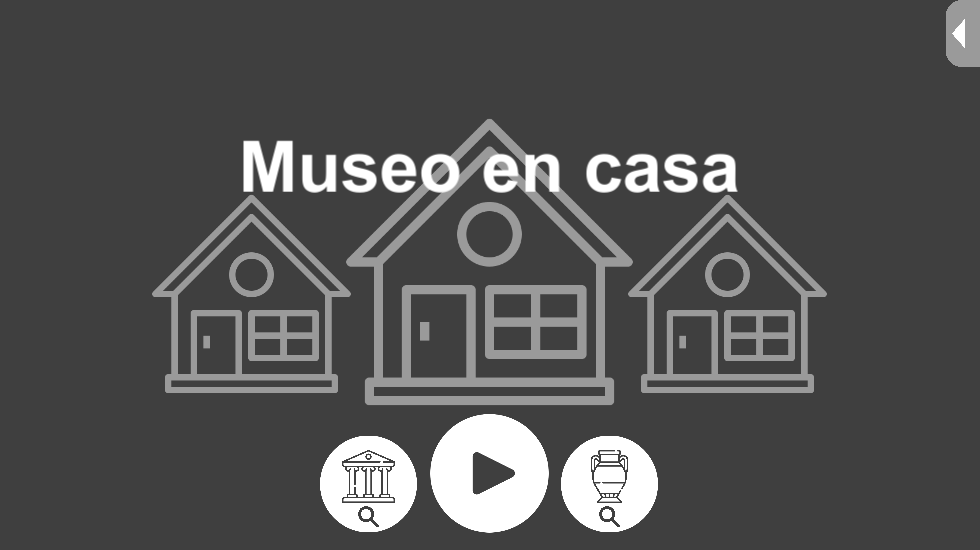
\includegraphics[width=15cm]{imgs/Game_2.PNG}}
\caption{Menu principal aplicación.}
\label{game_2}
\end{figure}

\begin{figure}[H]
\centerline{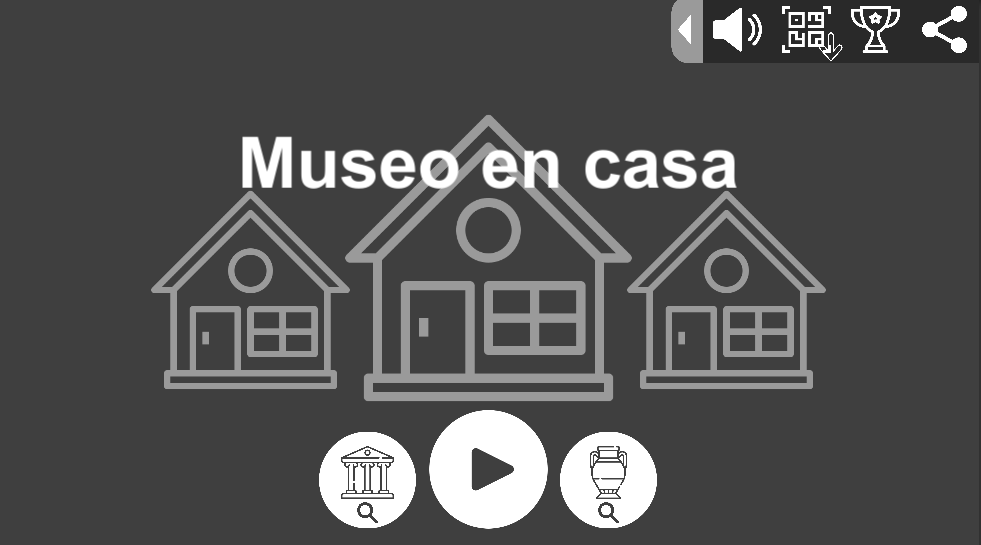
\includegraphics[width=15cm]{imgs/Game_1.PNG}}
\caption{Menu principal aplicación con menu de opciones desplegado.}
\label{game_1}
\end{figure}

\begin{figure}[H]
\centerline{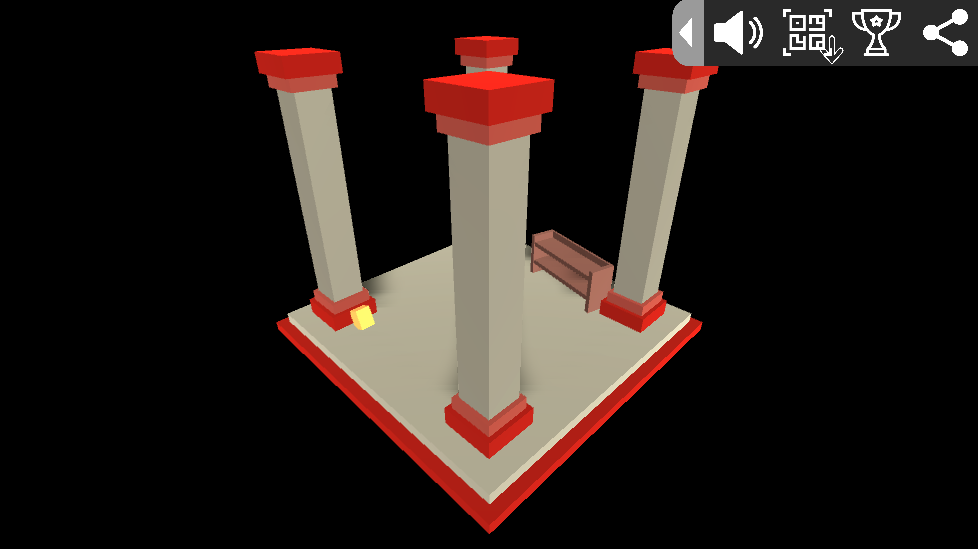
\includegraphics[width=15cm]{imgs/Game_4.PNG}}
\caption{Escena de juego mostrando una habitación del museo.}
\label{game_4}
\end{figure}

\begin{figure}[H]
\centerline{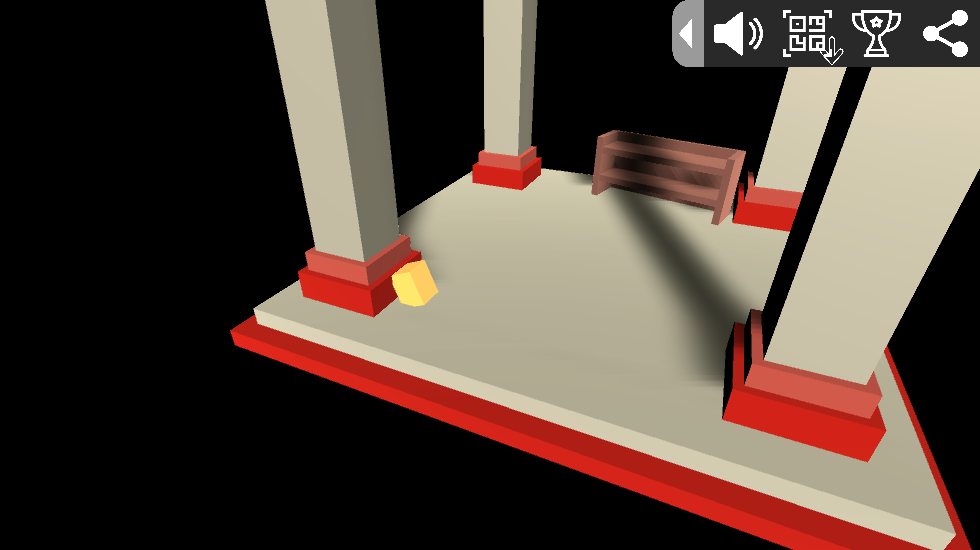
\includegraphics[width=15cm]{imgs/Game_5.PNG}}
\caption{Acercamiento a pieza a descubrir del museo.}
\label{game_5}
\end{figure}

\begin{figure}[H]
\centerline{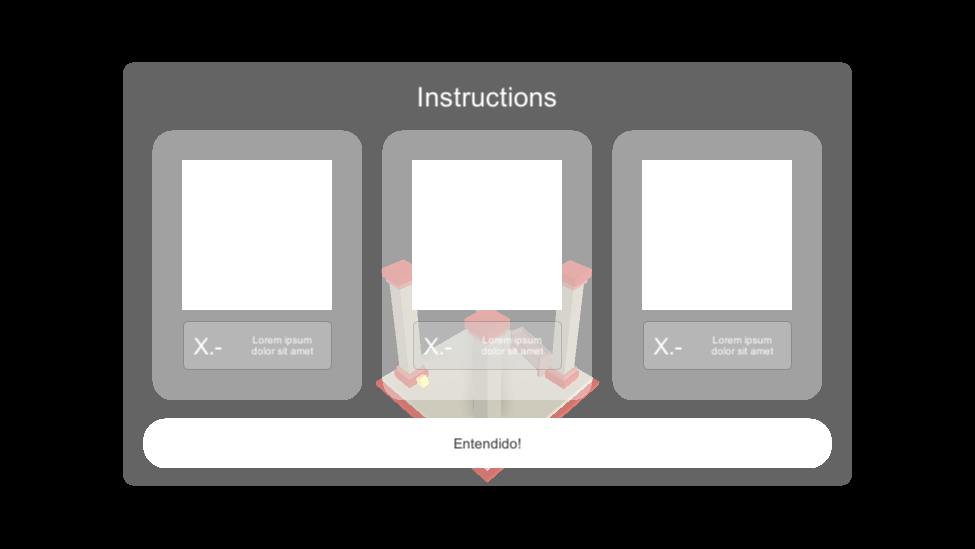
\includegraphics[width=15cm]{imgs/Game_3.PNG}}
\caption{Escena de juego mostrando pantalla de tutorial.}
\label{game_3}
\end{figure}

%%%%%%%%%%% DISEÑO %%%%%%%%%%%%%
%%%% Latex no permite el uso de 3 subsection por lo que \paragraph fue modificado para que cumpla con las caracteristicas de una subsection

\newpage
\section{Diseño}

\subsection{Derivación del Modelo de Software}
\subsubsection{Modelo de software inicial}
\subsubsection{Diagramas de Clases}
\subsubsection{Diagramas de Interacción}
\subsubsection{Diagramas de Estados}

\subsection{Refinamientos}
\subsubsection{Lugar de Refinamiento}
\subsubsection{Para cada Lugar}
\paragraph{Refinamientos considerados}
\paragraph{Selección y descripción de una opción}

%%%%%%%%%%%%%% IMPLEMENTACION %%%%%%%%%%
\newpage
\section{Implementación}

\subsection{Código fuente completo (parcial)}
El código de la app se hizo en base al diagrama UML presentado anteriormente, este se encuentra en un repositorio de github el cual se encuentra público para la revisión completa de este.

El código contiene tanto bibliotecas externas, como los scripts creados por el equipo de programación. 

\href{https://github.com/pokelocos/Prototipo_Ing_Software/tree/master/repo_ingSoftware}{Repositorio del Prototipo de `Museo en Casa'. (Hacer Click en el texto para ir al link)}



\subsection{Dependencias}

\begin{itemize}

\item Vuforia: Se utilizo esta librería para implementar las funcionalidades de Realidad Aumentada dentro del motor gráfico Unity.

\item Android SDK: Se utilizo esta SDK para realizar los builds para los dispositivos de Android.

\item Unity Engine package: Se utilizo esta librería para todas las funcionalidades que eran necesarias para la app, ya sea interacción con la UI, elementos del juego, etc.

\item Native Share for Android & iOS: Se utilizo esta librería para poder compartir las piezas de museos que hayan sido descubiertas por los usuarios de la app.


\end{itemize}

%%%%%%%%%%%%%%%% ANEXOS %%%%%%%%%%%%%%%%5
\newpage
\section{Anexos}


%\newglossaryentry{gls-EI} {
%  name={Entrada externa},
%  description={Corresponden a los datos entregados a la aplicación.},
%}
%\newacronym[longplural={Entrada externa}]{EI_Label}{EI}{Entrada externa}

%\gls{EI_Label}


\subsection{Glosario}



\begin{enumerate}
	\item \textbf{APP:} Acrónimo de aplicación.
	\item \textbf{Codificación:} Acción de generar código de programación.
	\item \textbf{DET:} Data Element Types, Son la cantidad de datos relacionados a un elemento de la aplicación.
	\item \textbf{EI:} Entrada externa, son los datos entregados a la aplicación.
	\item \textbf{EO:} Salida externa, son los datos entregados por la aplicación.
	\item \textbf{EQ:} Consulta externa, hace referencia a las consultas que realice la aplicación a otros sistemas.
	\item \textbf{EIF:} Ficheros de interfaces externas, grupo de datos relacionados lógicamente, se mantienen fuera de la aplicación.
	\item \textbf{FTR:} File Type Referenced, son la cantidad de conecciones a los diferentes grupos de datos.
	\item \textbf{FP:} Function points, es el valor de medida entregado por las funcionalidades de una aplicación, están ayudan a definir la complejidad de un proyecto.
	\item \textbf{HH:} Horas hombre, es una unidad de medida para medir el esfuerzo de un trabajo según las horas de trabajo por persona.
	\item \textbf{ILF:} Ficheros lógicos internos, grupo de datos relacionados lógicamente, se mantienen dentro de la aplicación.
	\item \textbf{LOC:} Lines of code, es una unidad de medida que denota el valor de un código por su cantidad de líneas.
	\item \textbf{Pieza, PH  o Pieza Histórica:} Es el nombre usado para referirse a los elementos del juego que representan a los propios elementos de los museos que están en exposición.
	\item \textbf{RRSS:} Acrónimo de redes sociales.
	\item \textbf{UI:} User Interface, es el tipo de vista que se ocupa en una aplicación que permite al usuario interactuar con la aplicación.
\end{enumerate}
















\end{document}
